\documentclass[12pt]{article}
\usepackage[a4paper, margin=2cm]{geometry}
\usepackage[english]{babel} % To obtain English text with the blindtext package
\usepackage{blindtext}
\usepackage{graphicx} % Required for inserting images
\usepackage{array} % For extra column formatting
\usepackage{amsmath} %for equation environment
\usepackage{float}
\usepackage{parskip} % For gaps between para
\usepackage{setspace}
\usepackage{pdfpages}
\usepackage{abstract}
\usepackage[export]{adjustbox}
\usepackage{emptypage}
\usepackage{tocloft}
\usepackage[nottoc]{tocbibind}
\usepackage{hyperref, url}
\usepackage{subcaption}
\usepackage{lipsum}
\usepackage{xcolor}


\cftsetindents{section}{0em}{2em}
\cftsetindents{subsection}{0em}{2em}

\renewcommand\cfttoctitlefont{\hfill\Large\bfseries}
\renewcommand\cftaftertoctitle{\hfill\mbox{}}

\graphicspath{ {./images/} }

\pagenumbering{arabic}

\definecolor{blurple}{HTML}{5865F2}

\hypersetup{
    colorlinks=true,
    linkcolor=black,
    urlcolor=blurple,
    citecolor=blurple,
}

\urlstyle{same}
%%%%%%%%%%%%%%%%%%%%%%%%%%%%%%%%%%%


\title{PHYC20090 Exp.7 LCR Circuits}
\author{Joana Adao}
\date{\today}

\begin{document}

\begin{titlepage}
    \begin{center}

        \begin{figure}[ht]
            
\includegraphics[width=\textwidth]{UCDLogo.png}
        \end{figure}
        
        \begin{figure}
            \centerline{
\includegraphics[width=\paperwidth]{UCDBanner.png}}
        \end{figure}

        \vspace{4cm}

        {\Huge \bfseries PHYC20090 Electronics and Devices}\\
        \vspace{0.75cm}
        {\LARGE Experiment No.7 Sinusodial Response of the LCR Resonant Circuit }
        
        \vspace{1cm}
    
    {\Large \textbf{27 January 2025 }}

    \vspace{2cm}
    
    {\large \textbf{by Joana C.C. Adao (Student No. 23311051)}}\\
    \medskip
    {\large With Arminas A., Ananya L., Samuel S.}

    \end{center}
    
   \clearpage

\end{titlepage}

\setcounter{page}{1}
\tableofcontents

\newpage

\begin{abstract}
\addcontentsline{toc}{section}{Abstract}

The aim of this experiment was to



\end{abstract}


%%%%%%%%%%%%%%%%%%%%%%%%%%%%%%%%%%%


\section{Theory}

\subsection{LCR Circuits} \label{sec:1.1}
An LCR circuit is made up of inductors (L), capacitors (C), and resistors (R), usually connected in series.
Since all the components of the circuit are connected in series, equal amount of the current will flow through each element.
\cite{unacademy}

A circuit containing these components, L, C, and R, can act as themselves individually at certain frequencies
\cite{learnabout}.
The LCR circuit can also magnify the voltages across the L, C, and R such that it is larger than the  circuit's input voltage (ie. AC, Alternating Current)
\cite{learnabout}.

\subsubsection{Inductance, Capacitance, Resistance} \label{sec:1.1.1}

Inductance, capacitance, and resistance make up the basic parameters that can affect circuits up to some degree
\cite{elecnotes}.

\textbf{Inductance} is a property of a conductor
\cite{britinductance}
and it's measured by its ability to store energy due to the magnetic field produced by the flow of current
\cite{elecnotes}
and the voltage that is induced by the current's rate of change
\cite{britinductance}.
With AC (Alternating Current), the magnetic field produced fluctuates with the time-varying properties of AC power sources
\cite{elecnotes,britinductance}.

The voltage is proportional to the rate of change of the current and this factor of proportionality is known as the inductance
\cite{britinductance}.
Coils of wire are most commonly used as the inductors in circuits as they amplify \cite{elecnotes} the efficiency at which the magnetic field induces
the voltage and current in the circuit. By coiling wire (solenoid) the magnetic field is concentrated and magnified at its centre, shown in Figure \ref{fig:solenoid}.

\begin{figure}[ht]
    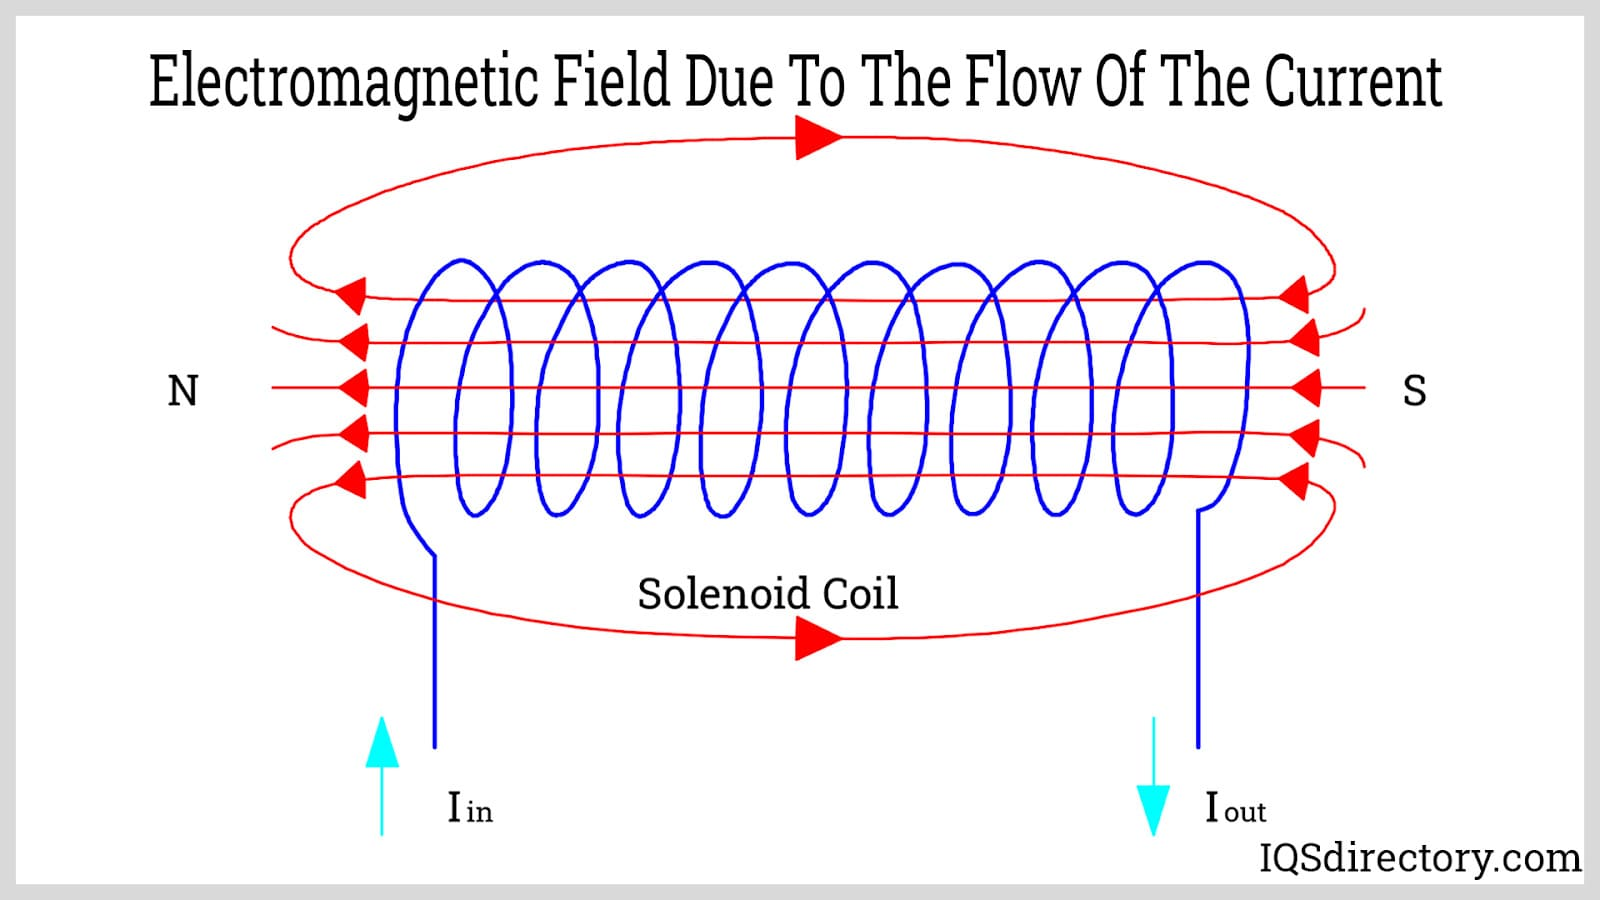
\includegraphics[width=15cm]{solenoid.jpg}
    \centering
    \caption{\centering Electromagnetic Field Due to the Flow of the Current in a Solenoid \cite{solenoidpic}}
    \label{fig:solenoid}
\end{figure}

\textbf{Capacitance} is a circuit's, or circuit component's, ability to collect and store electric charge
\cite{flukecapacitance}.
Capacitors are made up of two electrically conductive plates separated by some distance. These two plates, when voltage is exchanged between them,
become equally charged such that one plate is negatively charged (-Q) and the other is positively charged (+Q)
\cite{britcapacitance,librecapacitance}.
Overall, the charge of the capacitor will be neutral as the equal charge from both plates (-Q, +Q) cancels out
\cite{librecapacitance} as in figure \ref{fig:ppcapacitor}.

In a circuit with an AC supply, the capacitor is alternatively charged and discahrged every half cycle, therefore the amount of total
stored charge in that capacitor depends on the frequency of the AC supply as it dictates how long it will charge for
\cite{britcapacitance}.

Capacitors are usually assembled with a dielectric material inbetween the two conductive plates
\cite{britcapacitance,flukecapacitance,librecapacitance}.
Dielectric materials are poor conductors of electric fields, therefore labelled as insulators 
\cite{britdielectric}.
The capacitance of a capacitor increases with a dielectric material as the electric field is decreased and in turn so is the voltage across the two plates
\cite{hyperdielectric}.
The capacitor ends up storing the same charge as if it were without a dielectric material but at a lower voltage, which is effective in reducing the possibilites of a circuit short
\cite{hyperdielectric}.

\begin{figure}[ht]
    \centering
    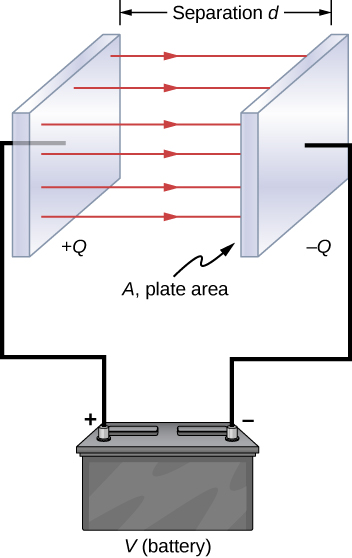
\includegraphics[width=5cm]{parallel plate capacitor.jpg}
    \caption{\centering Parallel Plate Capacitor Diagram \protect\cite{librecapacitance}}
    \label{fig:ppcapacitor}
\end{figure}

\textbf{Resistance} is a force that opposes the flow of current in a circuit
\cite{flukeresistance,hiokiresistance,britresistance}.
It can be described as the electrical charge's difficulty in moving through a material.
\cite{hiokiresistance}
Conductors and insulators, mentioned before, are types of materials classified by their resistance. Conductors are materials with little resistance that the
electrons can travel through easily, like copper and gold (most metals). Insulators, on the other hand, are materials that make it difficult for the electrical
charge to pass through, like wood and rubber
\cite{flukeresistance}.
These properties can be seen in electrical wires, with the current-carrying copper wire is encased in an insulating rubber tube for safety.

The resistance of a circuit component usually increases with temperature as the atoms that make up that material get excited, moving around in ways that make it
difficult for the electrons to travel through
\cite{britresistance,bbcresistance}.

Resistors are circuit components specifically made to counteract the flow of current in a circuit
\cite{britresistor,bbcresistance,hiokiresistance} (Figure).
Resistors can be used in a circuit to control the amount of voltage and current flowing in a circuit, which is useful to make sure the circuit doesn't blow and also
to correctly distribute the current/voltage throughout the circuit
\cite{britresistor,hiokiresistance}
The surplus of electrical energy flowing through a resistor is converted into heat energy which then dissipates
\cite{hiokiresistance}.

\begin{figure}[ht]
    \centering
    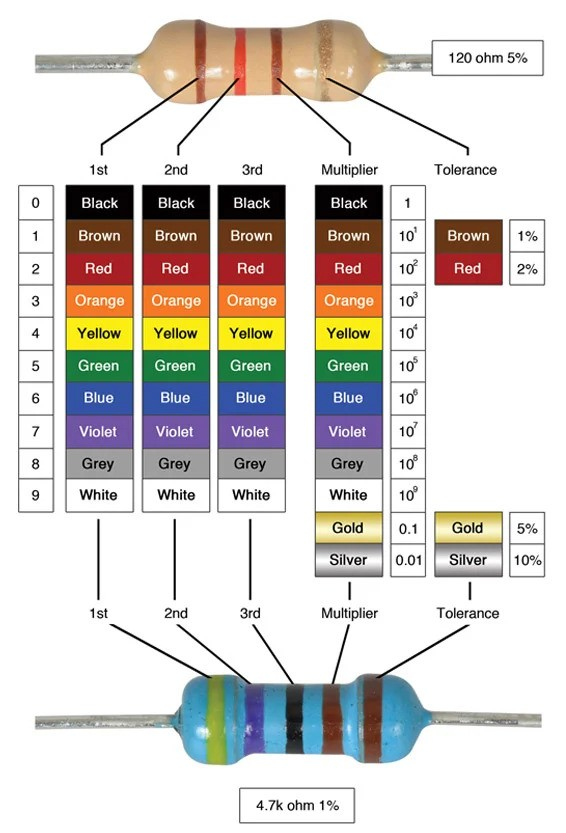
\includegraphics[width=7.5cm]{resistorr.jpg}
    \caption{\centering Resistor and How to Read One \protect\cite{resistorpic}}
    \label{fig:resistor}
\end{figure}

\subsubsection{Impedance} \label{sec:1.1.2}

The impedance of a circuit represents the overall resistance that it offers to AC
\cite{lionimpedance}.
The difference between resistance and impedance is that impedance only truly affects AC circuits while resistance affects both AC and DC (Direct Current)
\cite{isaacimpedance,protimpedance}.
In AC circuits the current is not constant but instead alternating, so the usual ratio of $\dfrac{V}{I}$ will also not be constant
\cite{isaacimpedance}.

Impedance is the vector sum of the resistance (R), when the current is in phase and peaks at the same time, and reactance (X), which peaks one quarter of the cycle,
within the circuit
\cite{lionimpedance,isaacimpedance}.
The reactance X is composed of the positive reactance of the inductor ($X_L$) and the negative reactance of the capacitor ($X_C$)
\cite{isaacimpedance}.

Impedance will be mathematically expanded on in §\ref{sec:1.3}, The Mathematics.

\subsection{Wave Properties} \label{sec:1.2}

Charged particles can create electromagnetic fields with their movement which transports
electromagnetic (EM) energy, like light and radiation.
They generate both an electric field and magnetic field, as the name implies
\cite{NASAemwave}.
Electromagnetic waves do need a material in order to be able to move, unlike mechanical waves
\cite{NASAemwave}.
As EM waves propagate, the frequency at which they're moving at has its own associated wavelength
\cite{NASAemradio}, as shown in figure \ref{fig:emrelation}. 
This is also how we can see colours, each frequency-associated wavelength is processed differently by our eyes,
which is actually a very narrow spectrum
\cite{emcolour}.

\begin{figure}[ht]
    \centering
    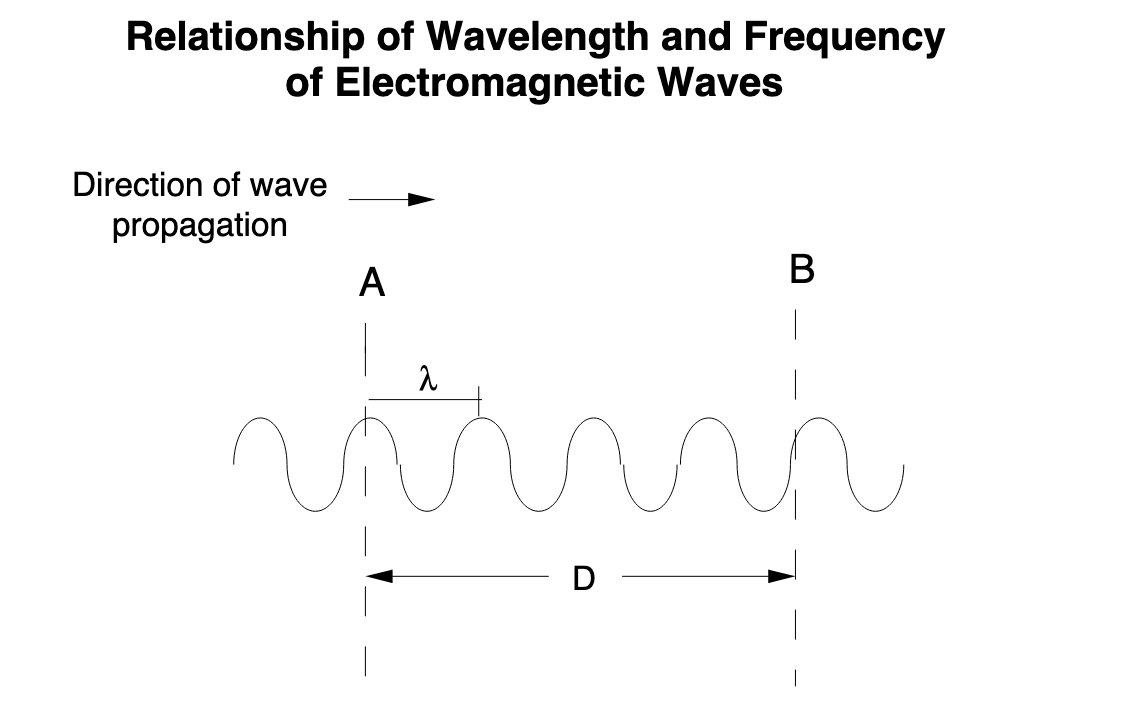
\includegraphics[width=15cm]{em wave relation.png}
    \caption{\centering Relationship of Wavelength and Frequency of Electromagnetic Waves \protect\cite{NASAemradio}}
    \label{fig:emrelation}
\end{figure}

\subsubsection{The Oscilloscope} \label{sec:1.2.1}

Oscilloscopes are device that display voltage as waves, typically sine waves, in order to visualise the variation of voltage over time
\cite{flukeoscillo,keyoscillo}.
The oscilloscope is an important device that will be used to find the resonant frequency of the LCR circuit being observed in the experiment.

\begin{figure}[ht]
    \centering
    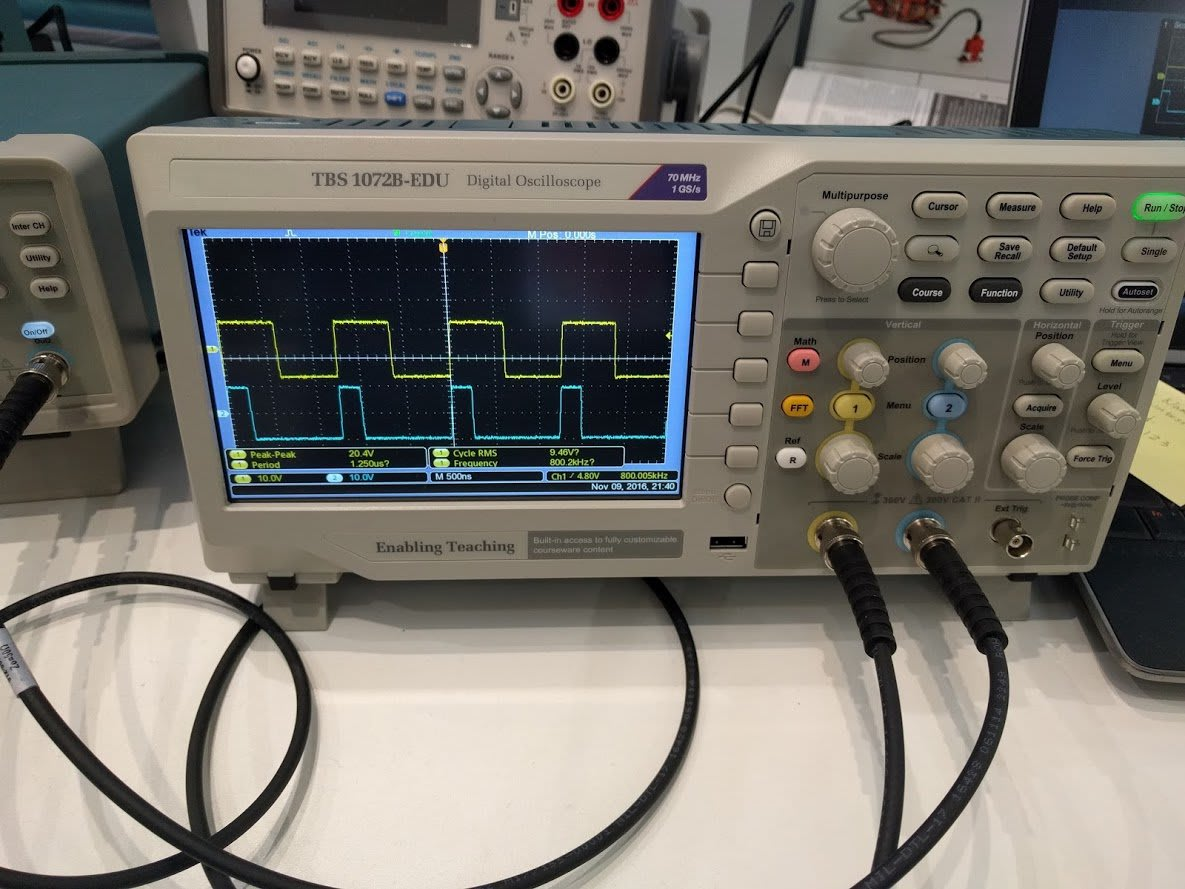
\includegraphics[width=10cm]{oscillo.jpg}
    \caption{\centering Oscilloscope With 2 Channels \protect\cite{oscillopic}}
\end{figure}

\subsubsection{Electrical Resonance} \label{sec:1.2.2}

Resonance in electrical circuits takes place at a specific, constant frequency at which the reactance and impedance cancel themselves out
\cite{geekresonance}.
The net reactance, in turn, is zero, so the current flow and voltage amplitude are increased
\cite{geekresonance}.

To get electrical resonance in a circuit the resonant frequency ($f_0$), at which the circuit is in resonance, must be found
\cite{geekresonance,eeresonance}.
Resonance, as a property of a wave, excites the particles of the same frequency. This is true even in electrical circuits.
When there net reactance is zero, the impedance in the circuit becomes entirely resistive so there is no counteraction to the flow of the current.
This constant resonance and increase in flow of current can lead to the circuit components overheating and breaking
\cite{geekresonance}.

Electical resonance will be mathematically expanded on in §\ref{sec:1.3}, The Mathematics.

\subsection{The Mathematics}\label{sec:1.3}

The reactance of the inductor $X_L$ is given by $\omega L$ where $\omega = 2 \pi f$, the angular frequency
\cite{UCD,isaacimpedance}.
The reactance of the capacitor $X_C$ is given by $- \dfrac{1}{\omega C}$ with $\omega$ once again as the angular frequency
\cite{UCD,isaacimpedance}.
Therefore, by understanding the total impedance formula is $\sqrt{R^2 + X^2}$
\cite{isaacimpedance},
we can then substitute X in for our two reactance values to get the impedance, Z:

\begin{gather} \label{eq:1}
    Z = \sqrt{R^2 + (X_L - X_C)^2}
\end{gather}

The current amplitude is given by $I = \dfrac{V}{Z}$, Ohm's Law, but for AC circuits extra considerations must be taken.
The AC equivalent to Ohm's Law occurs when $X_L = X_C$, where Z is then minimsed and thus the circuit will be in resonance (as discussed in §\ref{sec:1.2})
\cite{UCD}.

The time domain and frequency domain are two representations of the LCR circuit, as show below in figure \ref{fig:timefreq}.

\begin{figure} [ht]
    \centering
    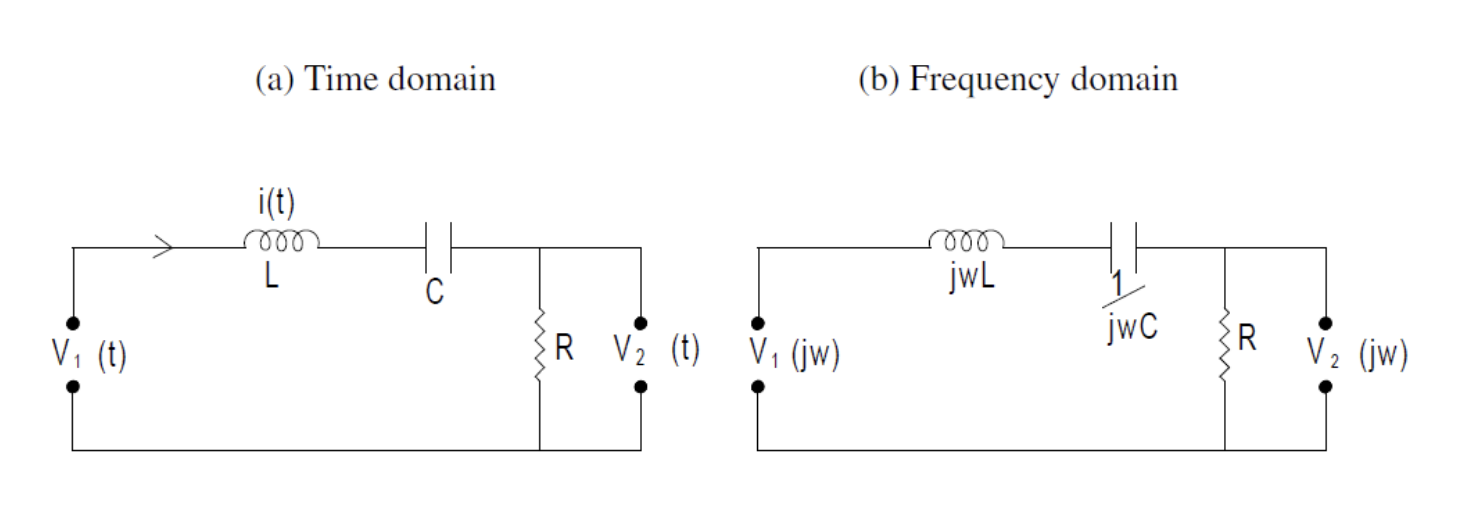
\includegraphics[width=\textwidth]{time and freq domains.png}
    \caption{\centering Time and Frequency Domains of the Series LCR Circuit \protect\cite{UCD}}
    \label{fig:timefreq}
\end{figure}

With the appropriate equations below the mathematical representation becomes clearer
\cite{UCD}.

Equation \ref{eq:2} represents Kirchoff's Voltage Law for series LCR circuits in the time domain, and equation \ref{eq:3} is the second-order differential equation
for the voltage that represents the time-varying response of the circuit (time domain).
Equation \ref{eq:4} is the phasor representation of the circuit in the frequency domain that takes into account the impedances from the capacitor and inductor,
as discussed in §\ref{sec:1.1.2}, the reactances. Equation \ref{eq:5} expresses the output voltage across the resistor in the frequency domain, and how the input voltage is
consequently transferred through the circuit.

\newpage
\hspace{2ex}
\begin{minipage}{0.45\textwidth}
    \begin{gather}
        v_1=L\frac{di}{dt}+\frac1C\int idt+R_1\label{eq:2}
    \end{gather}
    \vspace{-1.5em}
    \begin{gather}
        \frac{d^2v_2}{dt^2} + \frac{R dv_2}{L dt} + \frac{1}{LC} v_2 = \frac{dv_1}{dt} \cdot \frac{R}{L}\label{eq:3}
    \end{gather}
\end{minipage}
\hspace{-1.5ex}
\begin{minipage}{0.45\textwidth}
    \begin{gather}
        V_1 = j \omega L I + \frac{I}{j \omega C} + RI\label{eq:4}
    \end{gather}
    \vspace{-1.5em}
    \begin{gather}\label{eq:5}
        V_2 = IR = \frac{R}{j \omega L + \frac{1}{j \omega C} + R} V_1
    \end{gather}
\end{minipage}

\textit{Equations \ref{eq:2} and \ref{eq:3} representations of time domain. Equations \ref{eq:4} and \ref{eq:5} representations of frequency domain.} \cite{UCD}

The use of complex (j) phasors in the frequency domain allows for the simplification of this above analysis by entirely removing
the need for the integro-differential equations that are in the time domain. $H(j \omega)$ is defined at the sinusoidal response function, 
the ratio of the output to the input phasor in the frequency, equation \ref{eq:6}:

\begin{gather} \label{eq:6}
    H (j \omega) = \frac{V_2}{V_1} = \frac{j \omega C R}{1 - \omega^2 L C + j \omega C R}
\end{gather}

\section{The Procedure}



\section{Results and Calculations}



\section{Conclusion}



\section{Applications of Electrical Resonance}




\newpage


%%%%%%%%%%%%%%%%%%%%%%%%%%%%%%%%%%%

\bibliographystyle{IEEEtran}
\bibliography{References}


\newpage

\section*{Appendix}
\addcontentsline{toc}{section}{Appendix}

\subsection*{Raw Data}
\addcontentsline{toc}{subsection}{Raw Data}

\listoffigures


\end{document}